\documentclass[11pt,a4paper]{article}

% ---------------------------------------------------------------
% Tipografia: Palatino, versalete, uma cor de destaque (bord\^o)
% Mesmo pre\^ambulo da lista de trabalho e energia.
% ---------------------------------------------------------------
\usepackage[utf8]{inputenc}
\usepackage[T1]{fontenc}
\usepackage[brazil]{babel}
\usepackage[sc,osf]{mathpazo}
\usepackage{microtype}
\usepackage[top=2.4cm, bottom=2.6cm, left=2.6cm, right=2.6cm]{geometry}
\usepackage{amsmath}
\usepackage{amssymb}
\usepackage{xcolor}
\usepackage{tcolorbox}
\tcbuselibrary{skins, breakable}
\usepackage{enumitem}
\usepackage{booktabs}
\usepackage{array}
\usepackage{tabularx}
\usepackage{multirow}
\usepackage{needspace}
\usepackage{hyperref}
\usepackage{graphicx}
\graphicspath{{figuras/}}
\usepackage{comment}
\usepackage{pdfpages}   % anexa as resolu\c{c}\~oes manuscritas no fim

\definecolor{vinho}{RGB}{122, 27, 42}
\definecolor{grafite}{RGB}{70, 70, 70}
\hypersetup{colorlinks=true, linkcolor=vinho, urlcolor=vinho}

\linespread{1.06}
\setlength{\parindent}{0pt}
\setlength{\parskip}{0.45em}

% ---------------------------------------------------------------
% Formata\c{c}\~ao das quest\~oes
% ---------------------------------------------------------------
\newcommand{\fonte}[1]{{\small\scshape\color{grafite}#1}}

\newenvironment{questao}[2]{%
  \needspace{6\baselineskip}
  \par\addvspace{1.6em}
  {\large\bfseries\color{vinho}Quest\~ao #1}\hfill #2\\[-0.55em]
  {\color{black!25}\rule{\linewidth}{0.4pt}}
  \par\nobreak\smallskip
}{\par\addvspace{0.4em}}

\newcommand{\parte}[1]{%
  \needspace{7\baselineskip}
  \vspace{1.8em}
  {\Large\bfseries #1}\\[-0.55em]
  {\color{black!30}\rule{\linewidth}{0.5pt}}
  \par\nobreak\smallskip
}

\newtcolorbox{painel}{blanker, breakable, left=12pt,
  borderline west={1.4pt}{0pt}{black!30},
  before skip=11pt, after skip=11pt}

% figura recortada do caderno oficial do INEP
\newcommand{\figuraoriginal}[2]{%
  \begin{center}
    \includegraphics[width=#1]{#2}
  \end{center}}

% refer\^encia bibliogr\'afica do enunciado, como na prova
\newcommand{\fontebib}[1]{{\raggedleft\scriptsize\color{grafite}#1\par}}

\setlist[enumerate,1]{label=\textbf{\Alph*)}, leftmargin=2em, nosep}

% ---------------------------------------------------------------
\begin{document}
% ---------------------------------------------------------------

\thispagestyle{empty}

{\scshape\color{vinho}cursinho solid\'ario \,\textperiodcentered\, f\'isica}\\[-0.5em]
{\color{vinho}\rule{\linewidth}{1.6pt}}\\[0.9em]
{\huge\bfseries Lista de Quest\~oes}\\[0.35em]
{\LARGE Termologia}\\[0.7em]
{\itshape\color{grafite}Dezoito quest\~oes de ENEM, de 2011 a 2025}
\hfill {\color{grafite}2026}\\[-0.3em]
{\color{black!30}\rule{\linewidth}{0.5pt}}

\vspace{1.0em}

\begin{painel}
\begin{itemize}[nosep, leftmargin=1.5em]
  \item Comece por Q3, Q7 e Q9: uma de calor sens\'ivel, uma de mudan\c{c}a de
        fase e uma de propaga\c{c}\~ao. Q5 e Q14 s\~ao as mais longas.
  \item \textbf{Propaga\c{c}\~ao de calor \'e o subtema que mais cai}: cinco
        das quinze quest\~oes de 2020 a 2025. Gases e termodin\^amica
        aparecem s\'o duas vezes nessas seis provas (Q14 e Q15) --- vale
        saber disso ao distribuir o tempo de estudo.
  \item \textbf{A Parte VI n\~ao veio das provas recentes}: entre 2020 e
        2025 n\~ao caiu \emph{nenhuma} quest\~ao de m\'aquina t\'ermica no
        2\textordmasculine{} dia. Ela cobre o lado conceitual do que a
        aula d\'a no Bloco 6 --- por que sempre sobra calor e o que
        limita o rendimento --- e por isso puxa de provas mais antigas.
  \item No fim tem o gabarito comentado.
\end{itemize}
\end{painel}

\newpage

{\renewcommand{\arraystretch}{1.25}
\begin{tabular}{@{}clll@{}}
  \multicolumn{4}{@{}l}{{\scshape\color{vinho}mapa da lista}}\\
  \addlinespace[2pt]
  \toprule
  \# & Prova & Tema & \\
  \midrule
  1  & ENEM 2025 \,\textperiodcentered\, Q130 & Termometria: sensor de platina (gr\'afico)   \\
  2  & ENEM 2025 \,\textperiodcentered\, Q124 & Dilata\c{c}\~ao: l\^amina bimet\'alica               \\
  3  & ENEM 2020 \,\textperiodcentered\, Q101 & $Q = mc\Delta T$ com pot\^encia (num\'erica)   \\
  4  & ENEM 2022 \,\textperiodcentered\, Q129 & Calor espec\'ifico e amplitude t\'ermica       \\
  5  & ENEM 2022 \,\textperiodcentered\, Q111 & Calor sens\'ivel, vaz\~ao e corrente el\'etrica  \\
  6  & ENEM 2020 \,\textperiodcentered\, Q92  & Ebuli\c{c}\~ao na panela de press\~ao              \\
  7  & ENEM 2023 \,\textperiodcentered\, Q95  & Calor latente de condensa\c{c}\~ao               \\
  8  & ENEM 2024 \,\textperiodcentered\, Q112 & Solidifica\c{c}\~ao e isolamento (tirinha)       \\
  9  & ENEM 2025 \,\textperiodcentered\, Q91  & Irradia\c{c}\~ao: independe de fluidos           \\
  10 & ENEM 2024 \,\textperiodcentered\, Q117 & Convec\c{c}\~ao no aquecedor solar               \\
  11 & ENEM 2023 \,\textperiodcentered\, Q117 & Condutividade t\'ermica de um copo           \\
  12 & ENEM 2021 \,\textperiodcentered\, Q111 & Ilha de calor: irradia\c{c}\~ao e convec\c{c}\~ao      \\
  13 & ENEM 2020 \,\textperiodcentered\, Q133 & Convec\c{c}\~ao no condensador da geladeira      \\
  14 & ENEM 2024 \,\textperiodcentered\, Q101 & Ciclo de Otto no diagrama $P$--$V$         \\
  15 & ENEM 2023 \,\textperiodcentered\, Q119 & Pneu esfriando a volume constante ($P \times T$) \\
  16 & ENEM 2011 \,\textperiodcentered\, Q66  & Motor: por que sempre sobra calor          \\
  17 & ENEM 2012 \,\textperiodcentered\, Q83  & O que limita a efici\^encia de um motor     \\
  \bottomrule
\end{tabular}}

\newpage

% ===================================================================
\parte{Parte I --- Temperatura, Escalas e Dilata\c{c}\~ao}
% ===================================================================

\begin{questao}{1}{\fonte{ENEM 2025 \,\textperiodcentered\, caderno amarelo \,\textperiodcentered\, Q130}}
A resist\^encia de um fio de platina pode ser usada para medir
temperaturas entre 0 $^\circ$C e 100 $^\circ$C e j\'a foi utilizada como
refer\^encia para a escala internacional de temperatura. Para um sensor
feito de platina, a rela\c{c}\~ao entre a resist\^encia e a temperatura pode
ser descrita por uma equa\c{c}\~ao do tipo $R(T) = A + BT$, em que $T$ \'e a
temperatura e $A$ e $B$ s\~ao constantes. O gr\'afico apresenta a
depend\^encia da resist\^encia em fun\c{c}\~ao da temperatura para cinco
diferentes sensores.

\figuraoriginal{0.62\linewidth}{enem2025_q130_sensores_platina}

Os sensores que apresentam maior sensibilidade s\~ao
\begin{enumerate}
  \item 1 e 2.
  \item 1 e 3.
  \item 2 e 3.
  \item 2 e 4.
  \item 2 e 5.
\end{enumerate}
\end{questao}

\begin{questao}{2}{\fonte{ENEM 2025 \,\textperiodcentered\, reaplica\c{c}\~ao \,\textperiodcentered\, Q124}}
Um termostato \'e um dispositivo sens\'ivel a varia\c{c}\~oes de temperatura
utilizado para evitar o superaquecimento de alguns ferros de passar
roupas. Um desses dispositivos \'e constitu\'ido por uma l\^amina
bimet\'alica de a\c{c}o e lat\~ao que faz um contato el\'etrico. Quando a
l\^amina atinge uma determinada temperatura, sofre deflex\~ao e esse
contato \'e aberto, conforme a figura.

\figuraoriginal{0.95\linewidth}{enem2025r_q124_lamina_bimetalica}

A deflex\~ao dessa l\^amina ocorre porque o lat\~ao, em rela\c{c}\~ao ao a\c{c}o,
apresenta
\begin{enumerate}
  \item menor coeficiente de dilata\c{c}\~ao t\'ermica.
  \item maior coeficiente de dilata\c{c}\~ao t\'ermica.
  \item menor condutividade t\'ermica.
  \item maior condutividade t\'ermica.
  \item menor calor espec\'ifico.
\end{enumerate}
\end{questao}

% ===================================================================
\parte{Parte II --- Calor Sens\'ivel}
% ===================================================================

\begin{questao}{3}{\fonte{ENEM 2020 \,\textperiodcentered\, caderno amarelo \,\textperiodcentered\, Q101}}
Mesmo para peixes de aqu\'ario, como o peixe arco-\'iris, a temperatura da
\'agua fora da faixa ideal (26 $^\circ$C a 28 $^\circ$C), bem como sua
varia\c{c}\~ao brusca, pode afetar a sa\'ude do animal. Para manter a
temperatura da \'agua dentro do aqu\'ario na m\'edia desejada, utilizam-se
dispositivos de aquecimento com termostato. Por exemplo, para um aqu\'ario
de 50 L, pode-se utilizar um sistema de aquecimento de 50 W otimizado
para suprir sua taxa de resfriamento. Essa taxa pode ser considerada
praticamente constante, j\'a que a temperatura externa ao aqu\'ario \'e
mantida pelas estufas. Utilize para a \'agua o calor espec\'ifico
4,0 kJ$\cdot$kg$^{-1}\cdot$K$^{-1}$ e a densidade 1 kg$\cdot$L$^{-1}$.

Se o sistema de aquecimento for desligado por 1 h, qual o valor mais
pr\'oximo para a redu\c{c}\~ao da temperatura da \'agua do aqu\'ario?
\begin{enumerate}
  \item 4,0 $^\circ$C
  \item 3,6 $^\circ$C
  \item 0,9 $^\circ$C
  \item 0,6 $^\circ$C
  \item 0,3 $^\circ$C
\end{enumerate}
\end{questao}

\begin{questao}{4}{\fonte{ENEM 2022 \,\textperiodcentered\, caderno amarelo \,\textperiodcentered\, Q129}}
A varia\c{c}\~ao da incid\^encia de radia\c{c}\~ao solar sobre a superf\'icie da
Terra resulta em uma varia\c{c}\~ao de temperatura ao longo de um dia
denominada amplitude t\'ermica. Edifica\c{c}\~oes e pavimenta\c{c}\~oes realizadas
nas \'areas urbanas contribuem para alterar as amplitudes t\'ermicas dessas
regi\~oes, em compara\c{c}\~ao com regi\~oes que mant\^em suas caracter\'isticas
naturais, com presen\c{c}a de vegeta\c{c}\~ao e \'agua, j\'a que o calor
espec\'ifico do concreto \'e inferior ao da \'agua. Assim, parte da
avalia\c{c}\~ao do impacto ambiental que a presen\c{c}a de concreto proporciona
\`as \'areas urbanas consiste em considerar a substitui\c{c}\~ao da \'area
concretada por um mesmo volume de \'agua e comparar as varia\c{c}\~oes de
temperatura devido \`a absor\c{c}\~ao da radia\c{c}\~ao solar nas duas situa\c{c}\~oes
(concretada e alagada). Desprezando os efeitos da evapora\c{c}\~ao e
considerando que toda a radia\c{c}\~ao \'e absorvida, essa avalia\c{c}\~ao pode ser
realizada com os seguintes dados:

\begin{center}
{\renewcommand{\arraystretch}{1.5}
\begin{tabular}{@{}lcc@{}}
  \toprule
   & Densidade $\left(\dfrac{\mathrm{kg}}{\mathrm{m}^3}\right)$
   & Calor espec\'ifico $\left(\dfrac{\mathrm{J}}{\mathrm{g}\ ^\circ\mathrm{C}}\right)$ \\
  \midrule
  \'Agua    & 1\,000 & 4,2 \\
  Concreto  & 2\,500 & 0,8 \\
  \bottomrule
\end{tabular}}
\end{center}

A raz\~ao entre as varia\c{c}\~oes de temperatura nas \'areas concretada e
alagada \'e mais pr\'oxima de
\begin{enumerate}
  \item 1,0.
  \item 2,1.
  \item 2,5.
  \item 5,3.
  \item 13,1.
\end{enumerate}
\end{questao}

\begin{questao}{5}{\fonte{ENEM 2022 \,\textperiodcentered\, caderno amarelo \,\textperiodcentered\, Q111}}
O manual de uma ducha el\'etrica informa que seus tr\^es n\'iveis de
aquecimento (morno, quente e superquente) apresentam as seguintes
varia\c{c}\~oes de temperatura da \'agua em fun\c{c}\~ao de sua vaz\~ao:

\begin{center}
{\renewcommand{\arraystretch}{1.4}
\begin{tabular}{@{}cccc@{}}
  \toprule
  \multirow{2}{*}{Vaz\~ao $\left(\dfrac{\mathrm{L}}{\mathrm{min}}\right)$}
    & \multicolumn{3}{c}{$\Delta T$ ($^\circ$C)} \\
  \cmidrule(l){2-4}
    & Morno & Quente & Superquente \\
  \midrule
  3 & 10 & 20 & 30 \\
  6 & 5  & 10 & 15 \\
  \bottomrule
\end{tabular}}
\end{center}

Utiliza-se um disjuntor para proteger o circuito dessa ducha contra
sobrecargas el\'etricas em qualquer n\'ivel de aquecimento. Por padr\~ao, o
disjuntor \'e especificado pela corrente nominal igual ao m\'ultiplo de
5 A imediatamente superior \`a corrente m\'axima do circuito. Considere que
a ducha deve ser ligada em 220 V e que toda a energia \'e dissipada
atrav\'es da resist\^encia do chuveiro e convertida em energia t\'ermica
transferida para a \'agua, que apresenta calor espec\'ifico de
$4{,}2\ \dfrac{\mathrm{J}}{\mathrm{g}\ ^\circ\mathrm{C}}$ e densidade de
$1\,000\ \dfrac{\mathrm{g}}{\mathrm{L}}$.

O disjuntor adequado para a prote\c{c}\~ao dessa ducha \'e especificado por:
\begin{enumerate}
  \item 60 A
  \item 30 A
  \item 20 A
  \item 10 A
  \item 5 A
\end{enumerate}
\end{questao}

% ===================================================================
\parte{Parte III --- Mudan\c{c}as de Fase}
% ===================================================================

\begin{questao}{6}{\fonte{ENEM 2020 \,\textperiodcentered\, caderno amarelo \,\textperiodcentered\, Q92}}
As panelas de press\~ao reduzem o tempo de cozimento dos alimentos por
elevar a temperatura de ebuli\c{c}\~ao da \'agua. Os usu\'arios conhecedores
do utens\'ilio normalmente abaixam a intensidade do fogo em panelas de
press\~ao ap\'os estas iniciarem a sa\'ida dos vapores.

Ao abaixar o fogo, reduz-se a chama, pois assim evita-se o(a)
\begin{enumerate}
  \item aumento da press\~ao interna e os riscos de explos\~ao.
  \item dilata\c{c}\~ao da panela e a desconex\~ao com sua tampa.
  \item perda da qualidade nutritiva do alimento.
  \item deforma\c{c}\~ao da borracha de veda\c{c}\~ao.
  \item consumo de g\'as desnecess\'ario.
\end{enumerate}
\end{questao}

\begin{questao}{7}{\fonte{ENEM 2023 \,\textperiodcentered\, caderno amarelo \,\textperiodcentered\, Q95}}
Em uma ind\'ustria aliment\'icia, para produ\c{c}\~ao de doce de leite,
utiliza-se um tacho de parede oca com uma entrada para vapor de \'agua a
120 $^\circ$C e uma sa\'ida para \'agua l\'iquida em equil\'ibrio com o vapor
a 100 $^\circ$C. Ao passar pela parte oca do tacho, o vapor de \'agua
transforma-se em l\'iquido, liberando energia. A parede transfere essa
energia para o interior do tacho, resultando na evapora\c{c}\~ao de \'agua e
consequente concentra\c{c}\~ao do produto.

No processo de concentra\c{c}\~ao do produto, \'e utilizada energia proveniente
\begin{enumerate}
  \item somente do calor latente de vaporiza\c{c}\~ao.
  \item somente do calor latente de condensa\c{c}\~ao.
  \item do calor sens\'ivel e do calor latente de vaporiza\c{c}\~ao.
  \item do calor sens\'ivel e do calor latente de condensa\c{c}\~ao.
  \item do calor latente de condensa\c{c}\~ao e do calor latente de
        vaporiza\c{c}\~ao.
\end{enumerate}
\end{questao}

\begin{questao}{8}{\fonte{ENEM 2024 \,\textperiodcentered\, caderno cinza \,\textperiodcentered\, Q112}}
A tirinha ilustra esquim\'os dentro de um iglu, habita\c{c}\~ao de formato
hemisf\'erico constru\'ida durante o inverno a partir de neve ou blocos de
gelo. Essa estrutura de constru\c{c}\~ao se justifica pelo fato de esse povo
habitar as regi\~oes mais setentrionais da Groenl\^andia, Canad\'a e Alasca.

\figuraoriginal{0.92\linewidth}{enem2024_q112_tirinha_iglu}

\fontebib{LAERTE. Dispon\'ivel em: https://artedafisicapibid.blogspot.com.
Acesso em: 4 dez. 2021 (adaptado).}

Na tirinha, a geladeira \'e necess\'aria para fazer gelo porque
\begin{enumerate}
  \item a temperatura interna do iglu \'e maior que a de solidifica\c{c}\~ao
        da \'agua.
  \item a umidade dentro do iglu dificulta o processo de mudan\c{c}a de fase
        da \'agua.
  \item o ar dentro do iglu \'e isolante t\'ermico, dificultando a perda de
        calor pela \'agua.
  \item a temperatura uniforme no interior do iglu impede as correntes de
        convec\c{c}\~ao.
  \item a press\~ao do ar no interior do iglu \'e baixa, dificultando a
        solidifica\c{c}\~ao da \'agua.
\end{enumerate}
\end{questao}

% ===================================================================
\parte{Parte IV --- Propaga\c{c}\~ao de Calor}
% ===================================================================

\begin{questao}{9}{\fonte{ENEM 2025 \,\textperiodcentered\, caderno amarelo \,\textperiodcentered\, Q91}}
\textbf{TEXTO I}

\begin{center}
\itshape
As mariposas\\[0.2em]
As mariposa, quando chega o frio\\
Fica dando volta em volta da l\^ampida pra se esquent\'a. [sic]
\end{center}

\fontebib{BARBOSA, A. \textbf{Reviva: Adoniran Barbosa}. S\~ao Paulo:
Som Livre, 2002 (fragmento).}

\textbf{TEXTO II}

As mariposas se aproximam das l\^ampadas atra\'idas pela luz, pois, sendo
basicamente criaturas noturnas, est\~ao adaptadas a seguir o brilho da
lua, em um processo conhecido como orienta\c{c}\~ao transversal. Assim, o
que o sambista Adoniran Barbosa, no Texto I, descreve n\~ao \'e a causa,
mas sim uma das consequ\^encias poss\'iveis dessa aproxima\c{c}\~ao. De fato, o
calor gerado pelas l\^ampadas, sobretudo as incandescentes, pode aquecer
as mariposas.

\fontebib{HERTZBERG, R. Por que as mariposas s\~ao t\~ao atra\'idas por
luzes fortes? \textbf{National Geographic}, nov. 2020 (adaptado).}

Nesse contexto, o processo de transfer\^encia de calor para as mariposas
que independe da presen\c{c}a de fluidos \'e a
\begin{enumerate}
  \item reflex\~ao.
  \item refra\c{c}\~ao.
  \item irradia\c{c}\~ao.
  \item dispers\~ao.
  \item convec\c{c}\~ao.
\end{enumerate}
\end{questao}

\begin{questao}{10}{\fonte{ENEM 2024 \,\textperiodcentered\, caderno cinza \,\textperiodcentered\, Q117}}
Aquecedores solares s\~ao equipamentos utilizados para o aquecimento de
\'agua pelo calor do Sol. S\~ao compostos por coletores solares, nos quais
ocorre o aquecimento da \'agua, e por um reservat\'orio t\'ermico, em que \'e
armazenada a \'agua quente para ser utilizada posteriormente. A figura
ilustra esquematicamente como funciona esse equipamento.

\figuraoriginal{0.72\linewidth}{enem2024_q117_aquecedor_solar}

\fontebib{5 dicas de instala\c{c}\~ao de aquecedor solar. Dispon\'ivel em:
https://instaline.com.br. Acesso em: 3 nov. 2023 (adaptado).}

O processo pelo qual ocorre transfer\^encia de calor dos coletores solares
para o reservat\'orio t\'ermico \'e a
\begin{enumerate}
  \item difus\~ao.
  \item absor\c{c}\~ao.
  \item condu\c{c}\~ao.
  \item irradia\c{c}\~ao.
  \item convec\c{c}\~ao.
\end{enumerate}
\end{questao}

\begin{questao}{11}{\fonte{ENEM 2023 \,\textperiodcentered\, caderno amarelo \,\textperiodcentered\, Q117}}
Uma cafeteria adotou copos fabricados a partir de uma composi\c{c}\~ao de
50\% de pl\'astico reciclado n\~ao biodegrad\'avel e 50\% de casca de caf\'e.
O copo \'e reutiliz\'avel e retorn\'avel, pois o material, semelhante a uma
cer\^amica, suporta a lavagem. Embora ele seja comercializado por um
pre\c{c}o considerado alto quando comparado ao de um copo de pl\'astico
descart\'avel, essa cafeteria possibilita aos clientes retornarem o copo
sujo e levarem o caf\'e quente servido em outro copo j\'a limpo e
higienizado. O material desse copo oferece tamb\'em o conforto de n\~ao
esquentar na parte externa.

\fontebib{Cafeteria adota copo reutiliz\'avel feito com casca de caf\'e.
Dispon\'ivel em: www.gazetadopovo.com.br. Acesso em: 5 dez. 2019
(adaptado).}

Quais duas vantagens esse copo apresenta em compara\c{c}\~ao ao copo
descart\'avel?
\begin{enumerate}
  \item Ter a durabilidade de uma cer\^amica e ser totalmente
        biodegrad\'avel.
  \item Ser t\~ao dur\'avel quanto uma cer\^amica e ter alta condutividade
        t\'ermica.
  \item Ser um mau condutor t\'ermico e aumentar o res\'iduo biodegrad\'avel
        na natureza.
  \item Ter baixa condutividade t\'ermica e reduzir o res\'iduo n\~ao
        biodegrad\'avel na natureza.
  \item Ter alta condutividade t\'ermica e possibilitar a degrada\c{c}\~ao do
        material no meio ambiente.
\end{enumerate}
\end{questao}

\begin{questao}{12}{\fonte{ENEM 2021 \,\textperiodcentered\, caderno amarelo \,\textperiodcentered\, Q111}}
Na cidade de S\~ao Paulo, as ilhas de calor s\~ao respons\'aveis pela
altera\c{c}\~ao da dire\c{c}\~ao do fluxo da brisa mar\'itima que deveria atingir
a regi\~ao de mananciais. Mas, ao cruzar a ilha de calor, a brisa
mar\'itima agora encontra um fluxo de ar vertical, que transfere para ela
energia t\'ermica absorvida das superf\'icies quentes da cidade,
deslocando-a para altas altitudes. Dessa maneira, h\'a condensa\c{c}\~ao e
chuvas fortes no centro da cidade, em vez de na regi\~ao de mananciais. A
imagem apresenta os tr\^es subsistemas que trocam energia nesse fen\^omeno.

\figuraoriginal{0.62\linewidth}{enem2021_q111_ilha_calor}

No processo de fortes chuvas no centro da cidade de S\~ao Paulo, h\'a dois
mecanismos dominantes de transfer\^encia de calor: entre o Sol e a ilha de
calor, e entre a ilha de calor e a brisa mar\'itima.

\fontebib{VIVEIROS, M. \textbf{Ilhas de calor afastam chuvas de
represas}. Dispon\'ivel em: www2.feis.unesp.br. Acesso em: 3 dez. 2019
(adaptado).}

Esses mecanismos s\~ao, respectivamente,
\begin{enumerate}
  \item irradia\c{c}\~ao e convec\c{c}\~ao.
  \item irradia\c{c}\~ao e irradia\c{c}\~ao.
  \item condu\c{c}\~ao e irradia\c{c}\~ao.
  \item convec\c{c}\~ao e irradia\c{c}\~ao.
  \item convec\c{c}\~ao e convec\c{c}\~ao.
\end{enumerate}
\end{questao}

\begin{questao}{13}{\fonte{ENEM 2020 \,\textperiodcentered\, caderno amarelo \,\textperiodcentered\, Q133}}
Os manuais de refrigerador apresentam a recomenda\c{c}\~ao de que o
equipamento n\~ao deve ser instalado pr\'oximo a fontes de calor, como
fog\~ao e aquecedores, ou em local onde incida diretamente a luz do sol. A
instala\c{c}\~ao em local inadequado prejudica o funcionamento do
refrigerador e aumenta o consumo de energia.

O n\~ao atendimento dessa recomenda\c{c}\~ao resulta em aumento do consumo de
energia porque
\begin{enumerate}
  \item o fluxo de calor por condu\c{c}\~ao no condensador sofre
        consider\'avel redu\c{c}\~ao.
  \item a temperatura da subst\^ancia refrigerante no condensador diminui
        mais rapidamente.
  \item o fluxo de calor promove significativa eleva\c{c}\~ao da temperatura
        no interior do refrigerador.
  \item a liquefa\c{c}\~ao da subst\^ancia refrigerante no condensador exige
        mais trabalho do compressor.
  \item as correntes de convec\c{c}\~ao nas proximidades do condensador
        ocorrem com maior dificuldade.
\end{enumerate}
\end{questao}

% ===================================================================
\parte{Parte V --- Gases, Trabalho e Primeira Lei}
% ===================================================================

\begin{questao}{14}{\fonte{ENEM 2024 \,\textperiodcentered\, caderno cinza \,\textperiodcentered\, Q101}}
O diagrama $P$--$V$ a seguir representa o ciclo de Otto para um motor de
combust\~ao interna, como os motores a gasolina ou a etanol, utilizados
nos autom\'oveis.

\figuraoriginal{0.58\linewidth}{enem2024_q101_ciclo_otto}

As etapas representadas no diagrama est\~ao descritas no quadro.

\begin{center}
{\renewcommand{\arraystretch}{1.25}\small
\begin{tabular}{@{}ccl@{}}
  \toprule
  Etapa & Processo & Descri\c{c}\~ao \\
  \midrule
  I   & 0 a 1 & Admiss\~ao isob\'arica da mistura ar-combust\'ivel no cilindro do motor. \\
  II  & 1 a 2 & Compress\~ao adiab\'atica da mistura. \\
  III & 2 a 3 & Introdu\c{c}\~ao de energia na forma de calor da combust\~ao. \\
  IV  & 3 a 4 & Expans\~ao adiab\'atica. \\
  V   & 4 a 1 & Libera\c{c}\~ao de energia na forma de calor. \\
  VI  & 1 a 0 & Libera\c{c}\~ao dos gases resultantes da combust\~ao. \\
  \bottomrule
\end{tabular}}
\end{center}

\fontebib{Dispon\'ivel em: www.mspc.eng.br. Acesso em: 24 fev. 2013
(adaptado).}

A transforma\c{c}\~ao da energia t\'ermica em energia \'util ocorre na etapa
\begin{enumerate}
  \item II.
  \item III.
  \item IV.
  \item V.
  \item VI.
\end{enumerate}
\end{questao}

\begin{questao}{15}{\fonte{ENEM 2023 \,\textperiodcentered\, caderno amarelo \,\textperiodcentered\, Q119}}
O manual de um autom\'ovel alerta sobre os cuidados em rela\c{c}\~ao \`a
press\~ao do ar no interior dos pneus. Recomenda-se que a press\~ao seja
verificada com os pneus frios (\`a temperatura ambiente). Um motorista,
desatento a essa informa\c{c}\~ao, realizou uma viagem longa sobre o asfalto
quente e, em seguida, verificou que a press\~ao $P_0$ no interior dos
pneus n\~ao era a recomendada pelo fabricante. Na ocasi\~ao, a temperatura
dos pneus era $T_0$. Ap\'os um longo per\'iodo em repouso, os pneus do
carro atingiram a temperatura ambiente $T$. Durante o resfriamento, n\~ao
h\'a altera\c{c}\~ao no volume dos pneus e na quantidade de ar no seu
interior. Considere o ar dos pneus um g\'as perfeito (tamb\'em denominado
g\'as ideal).

Durante o processo de resfriamento, os valores de press\~ao em rela\c{c}\~ao
\`a temperatura ($P \times T$) s\~ao representados pelo gr\'afico:

\figuraoriginal{0.93\linewidth}{enem2023_q119_grafico_pxt}
\end{questao}

\newpage

% ===================================================================
\parte{Parte VI --- M\'aquinas T\'ermicas e Rendimento}
% ===================================================================

\begin{questao}{16}{\fonte{ENEM 2011 \,\textperiodcentered\, caderno azul \,\textperiodcentered\, Q66}}
Um motor s\'o poder\'a realizar trabalho se receber uma quantidade de
energia de outro sistema. No caso, a energia armazenada no combust\'ivel
\'e, em parte, liberada durante a combust\~ao para que o aparelho possa
funcionar. Quando o motor funciona, parte da energia convertida ou
transformada na combust\~ao n\~ao pode ser utilizada para a realiza\c{c}\~ao de
trabalho. Isso significa dizer que h\'a vazamento da energia em outra
forma.

De acordo com o texto, as transforma\c{c}\~oes de energia que ocorrem durante
o funcionamento do motor s\~ao decorrentes de a
\begin{enumerate}
  \item libera\c{c}\~ao de calor dentro do motor ser imposs\'ivel.
  \item realiza\c{c}\~ao de trabalho pelo motor ser incontrol\'avel.
  \item convers\~ao integral de calor em trabalho ser imposs\'ivel.
  \item transforma\c{c}\~ao de energia t\'ermica em cin\'etica ser
        imposs\'ivel.
  \item utiliza\c{c}\~ao de energia potencial do combust\'ivel ser
        incontrol\'avel.
\end{enumerate}
\end{questao}

\begin{questao}{17}{\fonte{ENEM 2012 \,\textperiodcentered\, caderno azul \,\textperiodcentered\, Q83}}
Aumentar a efici\^encia na queima de combust\'ivel dos motores a combust\~ao
e reduzir suas emiss\~oes de poluentes \'e a meta de qualquer fabricante de
motores. \'E tamb\'em o foco de uma pesquisa brasileira que envolve
experimentos com plasma, o quarto estado da mat\'eria e que est\'a presente
no processo de igni\c{c}\~ao. A intera\c{c}\~ao da fa\'isca emitida pela vela de
igni\c{c}\~ao com as mol\'eculas de combust\'ivel gera o plasma que provoca a
explos\~ao liberadora de energia que, por sua vez, faz o motor funcionar.

\fontebib{Dispon\'ivel em: www.inovacaotecnologica.com.br. Acesso em:
22 jul. 2010 (adaptado).}

No entanto, a busca da efici\^encia referenciada no texto apresenta como
fator limitante
\begin{enumerate}
  \item o tipo de combust\'ivel, f\'ossil, que utilizam. Sendo um insumo
        n\~ao renov\'avel, em algum momento estar\'a esgotado.
  \item um dos princ\'ipios da termodin\^amica, segundo o qual o
        rendimento de uma m\'aquina t\'ermica nunca atinge o ideal.
  \item o funcionamento c\'iclico de todos os motores. A repeti\c{c}\~ao
        cont\'inua dos movimentos exige que parte da energia seja
        transferida ao pr\'oximo ciclo.
  \item as for\c{c}as de atrito inevit\'avel entre as pe\c{c}as. Tais for\c{c}as
        provocam desgastes cont\'inuos que com o tempo levam qualquer
        material \`a fadiga e ruptura.
  \item a temperatura em que eles trabalham. Para atingir o plasma, \'e
        necess\'aria uma temperatura maior que a de fus\~ao do a\c{c}o com que
        se fazem os motores.
\end{enumerate}
\end{questao}

\newpage

% ===================================================================
\parte{Gabarito Comentado}
% ===================================================================

\begin{center}
{\renewcommand{\arraystretch}{1.25}
\begin{tabular}{cccccccc}
  \toprule
  1 & 2 & 3 & 4 & 5 & 6 & 7 & 8 \\
  \midrule
  E & B & C & B & B & B & E & D \\
  \bottomrule
\end{tabular}\\[0.7em]
\begin{tabular}{cccccccc}
  \toprule
  9 & 10 & 11 & 12 & 13 & 14 & 15 & 16 \\
  \midrule
  A & C & E & D & A & E & C & E \\
  \bottomrule
\end{tabular}\\[0.7em]
\begin{tabular}{cc}
  \toprule
  17 & 18 \\
  \midrule
  C & B \\
  \bottomrule
\end{tabular}}
\end{center}

\medskip

\begin{description}[style=nextline, leftmargin=0pt]

\item[Q1 --- E (sensibilidade \'e a inclina\c{c}\~ao).]
Sensibilidade \'e quanto a resist\^encia responde \`a temperatura, ou seja
$\mathrm{d}R/\mathrm{d}T = B$: a \textbf{inclina\c{c}\~ao} da reta. O sensor 2
sobe de cerca de 75 $\Omega$ a $-50\ ^\circ$C para 225 $\Omega$ a
320 $^\circ$C, a maior de todas; o sensor 5 vem em seguida (de ~65 para
~145 $\Omega$). O sensor 1 \'e praticamente horizontal --- resist\^encia
alta, mas sensibilidade quase nula, que \'e a pegadinha.

\item[Q2 --- B (a l\^amina encurva para o lado que dilata menos).]
Os dois metais sofrem o \textbf{mesmo} $\Delta T$, mas n\~ao dilatam
igual: o lat\~ao tem coeficiente de dilata\c{c}\~ao maior que o a\c{c}o
($\alpha \approx 19 \times 10^{-6}$ contra $12 \times 10^{-6}\
^\circ$C$^{-1}$). A face de lat\~ao fica mais comprida, a l\^amina se
encurva para o lado do a\c{c}o e o contato abre. Condutividade e calor
espec\'ifico n\~ao deformariam nada.

\item[Q6 --- E (o patamar n\~ao sobe com mais chama).]
A v\'alvula mant\'em a press\~ao interna constante e, com ela, a temperatura
de ebuli\c{c}\~ao. Depois que o vapor come\c{c}a a sair, aumentar a chama
\textbf{n\~ao eleva a temperatura}: s\'o evapora mais \'agua e gasta mais
g\'as. \'E exatamente o patamar da mudan\c{c}a de fase --- mais calor por
segundo significa fervura mais r\'apida, n\~ao mais quente.

\item[Q7 --- D (a origem, n\~ao o destino).]
Separe os dois lados da parede. \textbf{Origem} (a jaqueta): o vapor
esfria de 120 para 100 $^\circ$C, que \'e calor \textbf{sens\'ivel}, e
depois condensa a 100 $^\circ$C, que \'e calor \textbf{latente de
condensa\c{c}\~ao}. \textbf{Destino} (dentro do tacho): essa energia evapora
a \'agua do doce, e a\'i sim \'e latente de vaporiza\c{c}\~ao. A pergunta \'e
sobre a origem. O erro cl\'assico \'e marcar E, misturando as duas pontas.

\item[Q8 --- A (dentro do iglu n\~ao est\'a abaixo de zero).]
A neve \'e um isolante t\'ermico excelente e o calor dos pr\'oprios corpos
aquece o ambiente: o interior fica \textbf{acima} de 0 $^\circ$C. Sem
estar abaixo do ponto de solidifica\c{c}\~ao, a \'agua n\~ao congela sozinha
--- da\'i a geladeira. As alternativas C e D descrevem propriedades reais
do iglu, mas nenhuma delas impede a \'agua de congelar se a temperatura
estivesse negativa.

\item[Q9 --- C (o \'unico que atravessa o v\'acuo).]
Condu\c{c}\~ao precisa de meio material e convec\c{c}\~ao precisa de um
\textbf{fluido} que se desloque. O \'unico modo que dispensa fluidos \'e a
\textbf{irradia\c{c}\~ao}. Reflex\~ao, refra\c{c}\~ao e dispers\~ao nem s\~ao modos
de transfer\^encia de calor --- s\~ao fen\^omenos \'opticos, e caem tr\^es
alternativas de uma vez.

\item[Q10 --- E (repare no trecho que a quest\~ao pede).]
Do Sol at\'e o coletor \'e irradia\c{c}\~ao --- e \'e isso que a maioria marca.
Mas a pergunta \'e \textbf{do coletor para o reservat\'orio}. Nesse trecho
o que se move \'e a pr\'opria \'agua quente, que sobe por ficar menos densa:
\'e \textbf{convec\c{c}\~ao} (termossif\~ao). Mat\'eria se deslocando em fluido.

\item[Q11 --- D (as duas metades t\^em de estar certas).]
Metade f\'isica, metade ambiental. N\~ao esquentar na parte externa
significa \textbf{baixa condutividade t\'ermica}; ser reutiliz\'avel
significa \textbf{reduzir o res\'iduo n\~ao biodegrad\'avel}, e o enunciado
diz na primeira linha que o pl\'astico \'e n\~ao biodegrad\'avel. As
distratoras trocam ``baixa'' por ``alta'' condutividade ou chamam o
material de biodegrad\'avel.

\item[Q12 --- A (irradia\c{c}\~ao e convec\c{c}\~ao, nessa ordem).]
Sol $\rightarrow$ ilha de calor: atravessa o v\'acuo e a atmosfera, \'e
\textbf{irradia\c{c}\~ao}. Ilha de calor $\rightarrow$ brisa mar\'itima: o
enunciado entrega de gra\c{c}a ao falar de ``fluxo de ar vertical'' --- ar
subindo \'e \textbf{convec\c{c}\~ao}. Vale amarrar com a Q4: a cidade
esquenta mais que o campo porque o concreto tem calor espec\'ifico baixo.

\item[Q13 --- E (o condensador precisa jogar calor fora).]
O condensador \'e a grade atr\'as da geladeira, e o trabalho dele \'e
transferir calor para o ar da cozinha. Com uma fonte de calor ao lado, o
ar em volta fica quente e as \textbf{correntes de convec\c{c}\~ao} que
levariam esse calor embora ficam prejudicadas. O compressor precisa
trabalhar mais, e o consumo sobe.

\item[Q14 --- C (a etapa que empurra o pist\~ao).]
A etapa III \'e onde a energia \textbf{entra} (calor da combust\~ao), n\~ao
onde ela vira trabalho --- \'e a distratora mais marcada. Na
\textbf{expans\~ao adiab\'atica} (IV) n\~ao h\'a troca de calor, $Q = 0$, e a
primeira lei d\'a
\[
  \Delta U = Q - W = -W ,
\]
ou seja, a energia interna do g\'as \textbf{vira trabalho} sobre o pist\~ao.
\'E a etapa que empurra o pist\~ao para baixo, e a \'area sob ela no diagrama
\'e o que o motor entrega.

\item[Q15 --- E (press\~ao e temperatura absoluta s\~ao proporcionais).]
O volume do pneu n\~ao muda e a quantidade de ar tamb\'em n\~ao: sobra
$P/T = $ constante. Ent\~ao $P$ e $T$ s\~ao \textbf{diretamente
proporcionais}, e o gr\'afico \'e um peda\c{c}o de \textbf{reta alinhada com
a origem}. Esfriando, o ponto desce por essa reta, de $(T_0,\,P_0)$ para
$(T,\,P)$ com $P < P_0$. A e B mant\^em a press\~ao --- isso seria
isob\'arico, e a\'i o pneu teria de mudar de volume; C \'e curva, que \'e a
cara de uma isot\'ermica em $P \times V$, gr\'afico errado; D faz a
press\~ao \emph{subir} enquanto o pneu esfria. A propor\c{c}\~ao s\'o vale em
\textbf{kelvin} --- por isso o eixo da prova est\'a em K.

\item[Q16 --- C (\'e a segunda lei, dita com outras palavras).]
``Vazamento da energia em outra forma'' \'e o calor rejeitado na fonte
fria. Nenhuma m\'aquina t\'ermica converte todo o calor recebido em
trabalho: sempre sobra $Q_f$, e por isso $\eta = W/Q_q$ nunca chega a 1.
N\~ao \'e defeito de projeto nem atrito --- \'e limite de princ\'ipio.

\item[Q17 --- B (o limite \'e de princ\'ipio, n\~ao de engenharia).]
Mesma ideia da Q16, agora com o texto do plasma como pano de fundo. As
alternativas A, D e E citam limita\c{c}\~oes reais (combust\'ivel acaba,
pe\c{c}a desgasta, material funde), mas nenhuma delas \'e o que
\emph{impede} o rendimento de chegar a 100\%. O que impede \'e a segunda
lei da termodin\^amica.

\end{description}

\newcommand{\tituloanexo}{%
  \thispagestyle{empty}%
  {\Large\bfseries Resolu\c{c}\~oes Passo a Passo}\\[-0.55em]
  {\color{black!30}\rule{\linewidth}{0.5pt}}\\[0.35em]
  {\small\itshape\color{grafite}Manuscritas, das quest\~oes de
  calor sens\'ivel (Q3, Q4 e Q5).}%
}

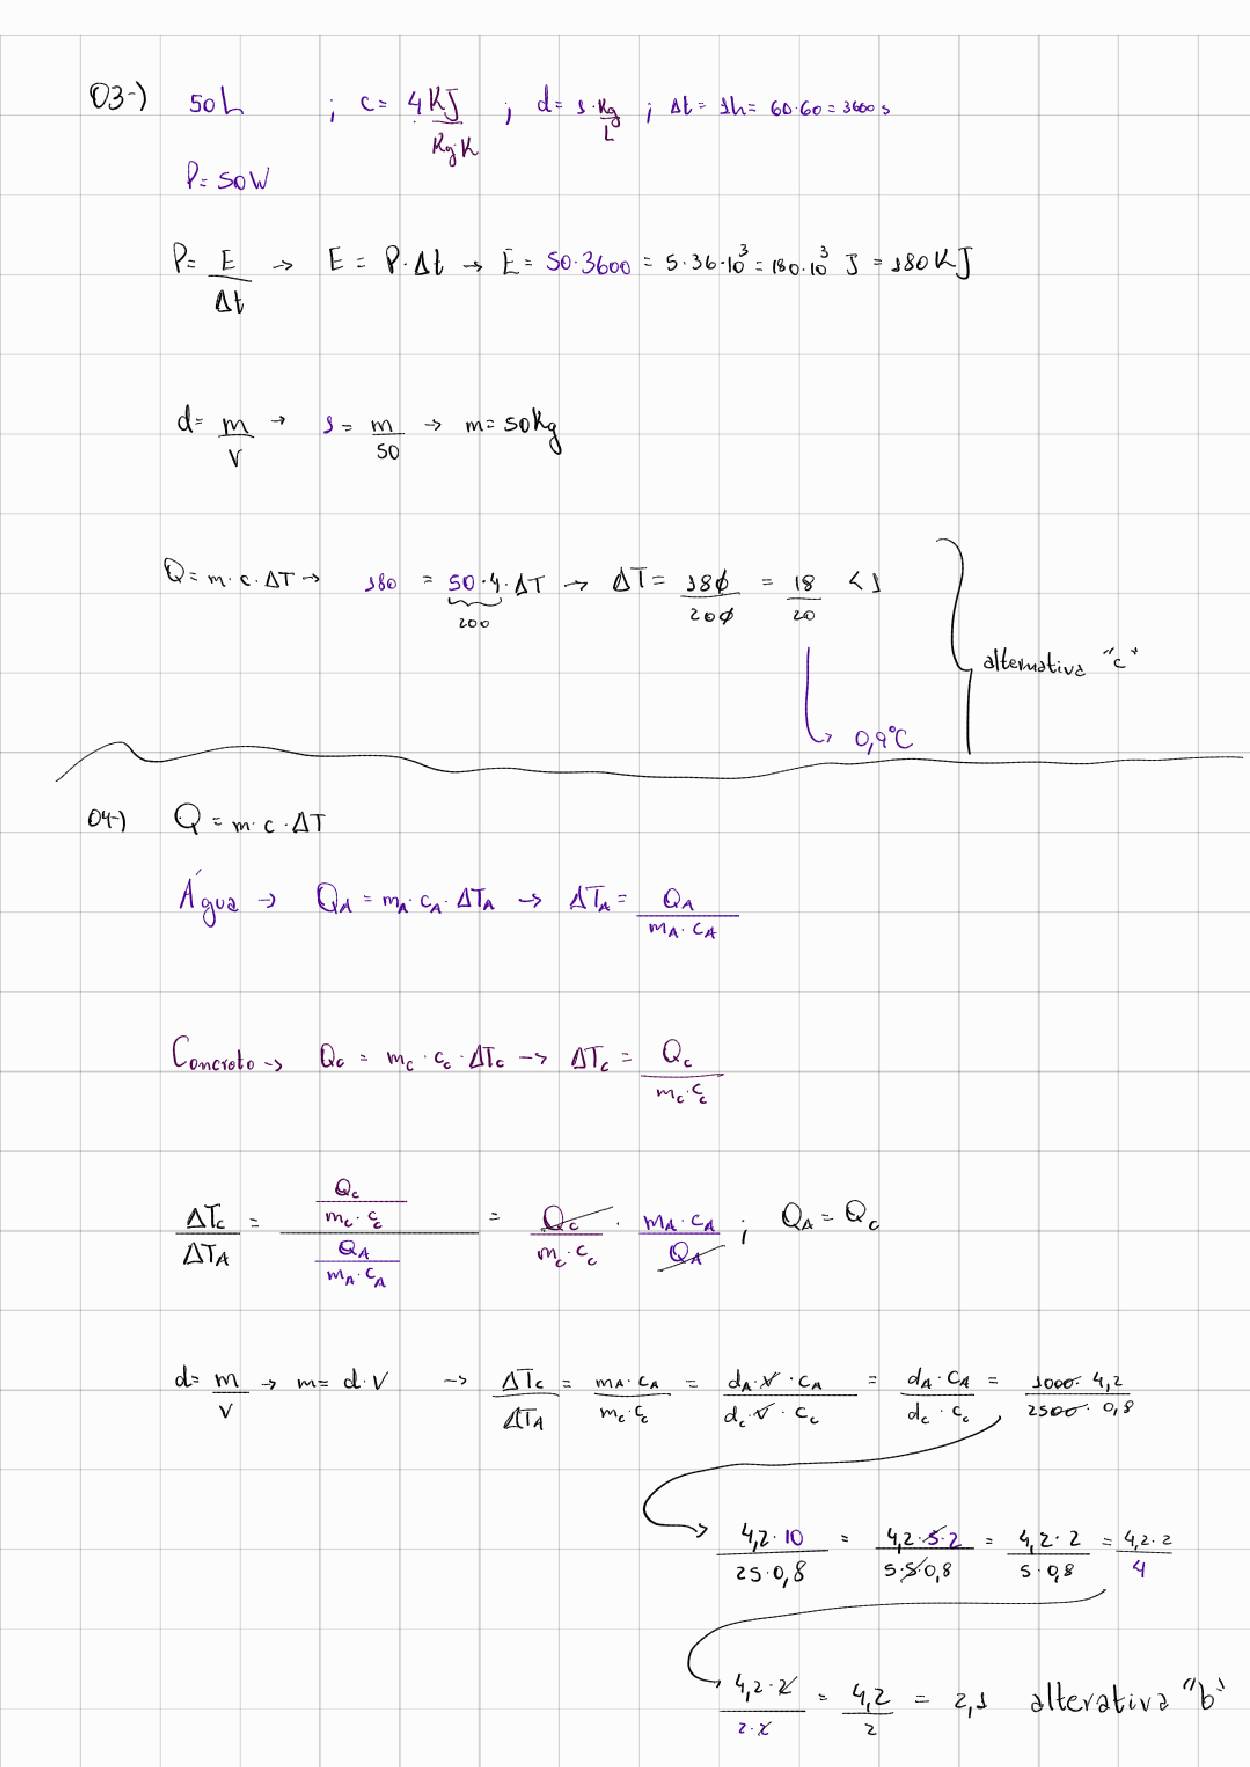
\includepdf[pages=1, scale=0.85, offset=0 -1.4cm,
  pagecommand=\tituloanexo]{resolucoes_termologia.pdf}

\includepdf[pages=2-, scale=0.95,
  pagecommand={\thispagestyle{empty}}]{resolucoes_termologia.pdf}

\bigskip

\begin{painel}
{\small\scshape\color{grafite}fontes}\par\smallskip
\small
\begin{itemize}[nosep, leftmargin=1.5em]
  \item \textbf{PDFs de origem}:
        \url{https://download.inep.gov.br/educacao_basica/enem/provas/}
        seguido de \texttt{ANO/ANO\_PV\_impresso\_D2\_CD5.pdf}
        (amarelo) ou \texttt{\_CD6.pdf} (cinza); a reaplica\c{c}\~ao de 2025 \'e
        \texttt{2025\_PV\_impresso\_D4\_CD5.pdf}.
  \item \textbf{Q16 e Q17 (m\'aquinas t\'ermicas)}: ENEM de 2011 e 2012,
        quando Ci\^encias da Natureza ainda ca\'ia no
        1\textordmasculine{} dia; numera\c{c}\~ao do caderno azul. Os
        enunciados vieram de compila\c{c}\~oes p\'ublicas dessas provas, e
        n\~ao do PDF do INEP, mas est\~ao na \'integra --- nenhuma das duas
        tem figura no original.
  \item \textbf{Sobre o gabarito}: as respostas acima foram obtidas
        a partir de resolu\c{c}\~oes passo a passo, que est\~ao
        no anexo final. A ordem das quest\~oes segue a do caderno oficial,
        caso haja divergência com o gabarito oficial do INEP, fico a disposição para esclarecimentos.
        
\end{itemize}
\end{painel}

\end{document}
